\documentclass{article}
\usepackage[utf8]{inputenc}
\usepackage{amsmath}
\usepackage{titlesec}
\usepackage{listings}
\usepackage[dvipsnames]{xcolor}

\usepackage{listings}
\lstloadlanguages{Ruby}
\lstset{%
basicstyle=\ttfamily\color{black},
commentstyle = \ttfamily\color{red},
keywordstyle=\ttfamily\color{blue},
stringstyle=\color{orange}}

\usepackage{hyperref}
\usepackage{indentfirst}
\titlelabel{\thetitle.\quad}
\usepackage{titling}
\usepackage{amssymb}
\usepackage{polski}
\usepackage[utf8]{inputenc}
\usepackage{minted}
\usepackage{pgfplots}
\newcommand{\subtitle}[1]{%
  \posttitle{%
    \par\end{center}
    \begin{center}\LARGE#1\end{center}
    \vskip0.5em}%
}

\pgfplotsset{compat=1.15}
\usepackage{mathrsfs}
\usetikzlibrary{arrows}
\usepackage[top=25mm, bottom=25mm,left=25mm,right=25mm]{geometry}
\title{\textbf{Uniwersytet Gdański
\\{\Large Wydział Matematyki, Fizyki i Informatyki}}}
\subtitle{Informatyka Ogólnoakademicka}
\author{Julia Komorowska}
\date{}
\begin{document}
\maketitle
\noindent 
\textit{Nr albumu}: 266386\newline\newline
\textit{Specjalność}: Ogólna \newline\newline
\textit{Rodzaj studiów}: Stacjonarne
\newline\newline
\normalsize
\newline\newline\newline\newline
\begin{center}
    {\LARGE\textbf{Testowanie klasyfikatorów na wybranej bazie danych}}\newline\newline
\end{center}


\begin{center}
\textbf{Gdańsk 2022}
\end{center}
\newpage
\begin{flushleft}
{\LARGE\textbf{Streszczenie}}
\end{flushleft}
{\large Zakres pracy obejmuje projekt polegający na testowaniu klasyfikatorów i porównaniu ich do siebie. Cała praca została także opisana w pliku:
\begin{itemize}
\item projekt.ipynb
\end{itemize}
Cały projekt został napisany w języku Python w Jupyter Notebook.}
\newline\newline\newline\newline
{\LARGE\textbf{Treść zadania}}
\newline\newline
{\large Celem projektu (typu d) jest przetestowanie klasyfikatorów na wybranej bazie danych. Można wybrać następującą bazę danych
\begin{itemize}
\item COVID19 \url{https://www.kaggle.com/einsteindata4u/covid19}
\end{itemize} 
}
\newpage
\normalsize
\newline
\tableofcontents
\normalsize
\newline\newline\newline\newline\newline\newline\newline\newline\newpage
\section{\LARGE{Wprowadzenie}}
\indent{\large Projekt został stworzony na podstawie bazy danych Covid-19 \url{https://www.kaggle.com/datasets/meirnizri/covid19-dataset}.}
\subsection{Importowanie paczek}
\newline\newline
\indent \large{Na początku trzeba zaimportować wszystkie paczki potrzebne do uruchomienia programu. }
\newline\newline
\begin{lstlisting}
from sklearn.linear_model import LinearRegression
from sklearn.neural_network import MLPClassifier
from sklearn import metrics
from sklearn.model_selection import train_test_split
from sklearn.metrics import accuracy_score, plot_confusion_matrix,precision_score,f1_score,recall_score
from sklearn.linear_model import Perceptron
from sklearn import tree
from sklearn.metrics import confusion_matrix,mean_squared_error, r2_score,classification_report
from sklearn.neighbors import KNeighborsClassifier
from sklearn.datasets import make_blobs
from sklearn.tree import export_graphviz,export_text
from sklearn.naive_bayes import GaussianNB,BernoulliNB,CategoricalNB
from sklearn.preprocessing import StandardScaler,OrdinalEncoder
import seaborn as sns
import numpy as np
import pandas as pd
import matplotlib.pyplot as plt
from six import StringIO
from IPython.display import Image  
import pydotplus
from mlxtend.preprocessing import TransactionEncoder
from mlxtend.frequent_patterns import apriori, association_rules
import warnings
import json
warnings.filterwarnings("ignore")
\end{lstlisting}
\newpage
\subsection{Preprocessing}
\indent{\large Wstępne przetwarzanie bazy danych w celu zapewnienia większej wydajności jest pierwszym krokiem do przygotowania naszej bazy danych do użytku.  }\newline\newline
\begin{itemize}

\item Pobranie bazy danych i pokazanie jej kolumn.
\begin{lstlisting}
df = pd.read_csv("covid_data.csv")
for col in df.columns:
    print(col)
\end{lstlisting}
\begin{center}
    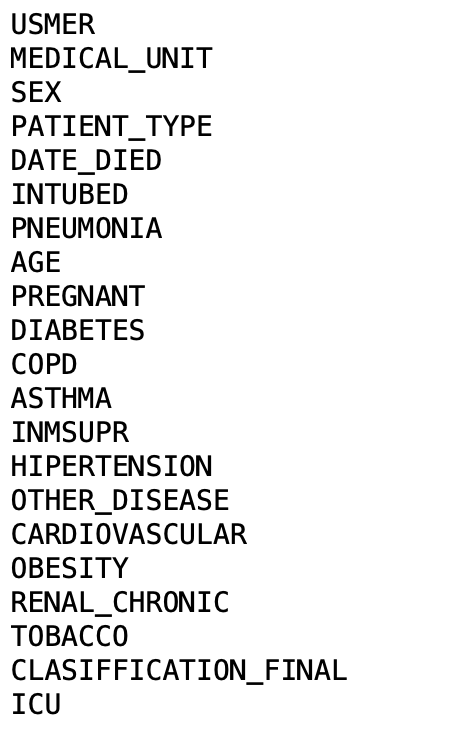
\includegraphics[width=0.4\textwidth]{image1.png}\newline
\end{center}
\item Jak widać po pierwszych pięciu wierszach i ostatnich baza danych jest niezrozumiała. Dobrym przykładem jest ciąża, jeśli dana osoba jest mężczyzną to wtedy kolumna \newline"PREGNANT" zawiera liczbe 97, a kiedy jest kobietą zawiera liczbę 2 lub 98 w zależności od tego czy jest w ciąży.
\begin{center}
    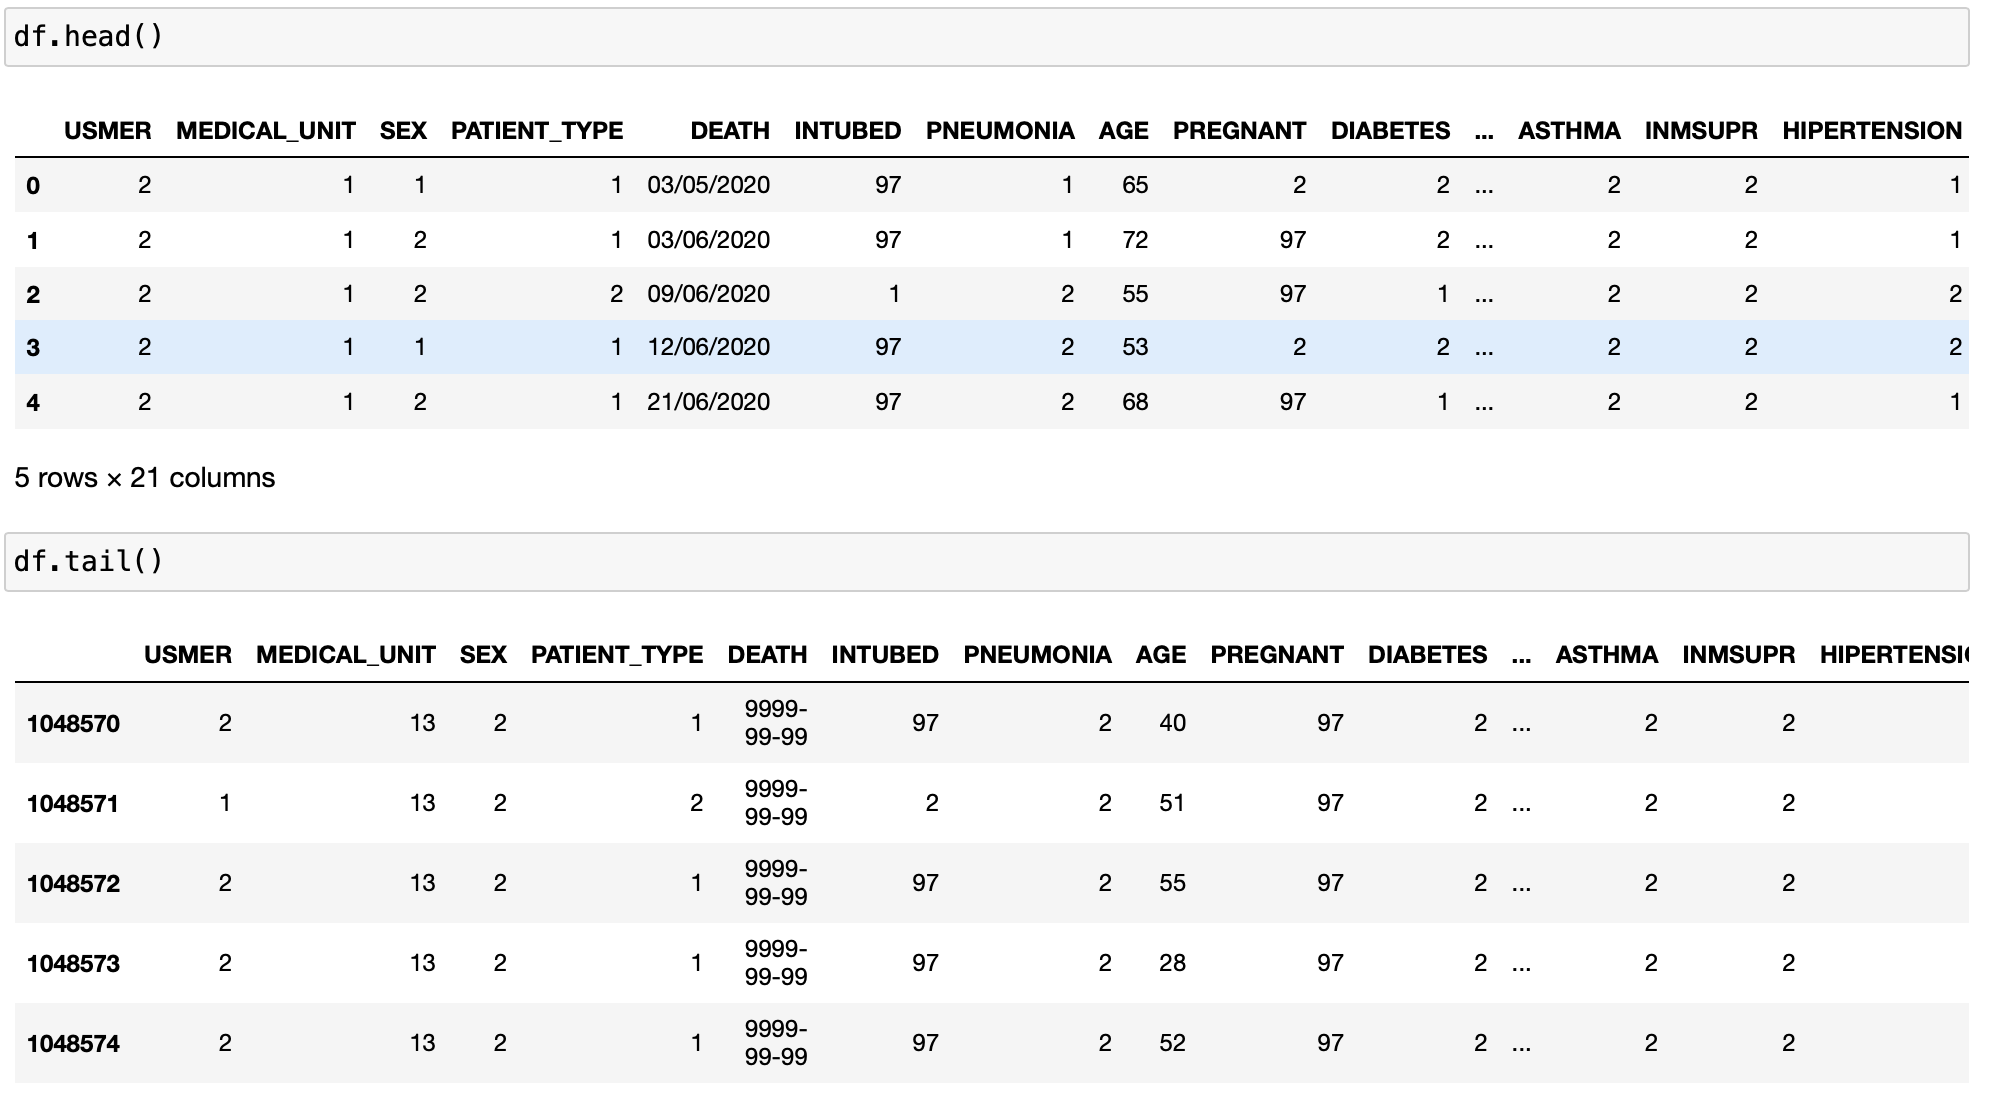
\includegraphics[width=1.0\textwidth]{image2.png}\newline
\end{center}
\item Zmiana nazw kolumn or usunięcie niepotrzebnych. Wartości zostały zmienione na wartości binarne.
\begin{lstlisting}
df.rename(columns= {'DATE_DIED':"DEATH"},inplace=True)


cols =['USMER','MEDICAL_UNIT','SEX','PATIENT_TYPE','DEATH','INTUBED','PNEUMONIA','AGE','PREGNANT','DIABETES',
          'COPD','ASTHMA','HIPERTENSION','OTHER_DISEASE',
          'CARDIOVASCULAR','OBESITY','RENAL_CHRONIC','TOBACCO']

          
def change(column,points,names=None):
    if not names:
        names= range(len(points)+1)
    colCut= pd.cut(column,bins = [column.min()]+ points+[column.max()],labels=names,include_lowest=True)
    return colCut

df['INTUBED']=change(df['INTUBED'],[90],[0,1])
df['PREGNANT']=change(df['PREGNANT'],[97],[0,1])
df['HIPERTENSION']=change(df['HIPERTENSION'],[90],[0,1])
df['PNEUMONIA']=change(df['PNEUMONIA'],[90],[0,1])
df['TOBACCO']=change(df['TOBACCO'],[90],[0,1])
df['OTHER_DISEASE']=change(df['OTHER_DISEASE'],[90],[0,1])
df['CARDIOVASCULAR']=change(df['CARDIOVASCULAR'],[90],[0,1])
df['OBESITY']=change(df['OBESITY'],[90],[0,1])
df['RENAL_CHRONIC']=change(df['RENAL_CHRONIC'],[90],[0,1])
df['ASTHMA']=change(df['ASTHMA'],[90],[0,1])
df['COPD']=change(df['COPD'],[90],[0,1])
df['DIABETES']=change(df['DIABETES'],[90],[0,1])

df = df.drop('INMSUPR', axis=1)
df = df.drop('CLASIFFICATION_FINAL', axis=1)
df = df.drop('ICU', axis=1)

\end{lstlisting}
\begin{center}
    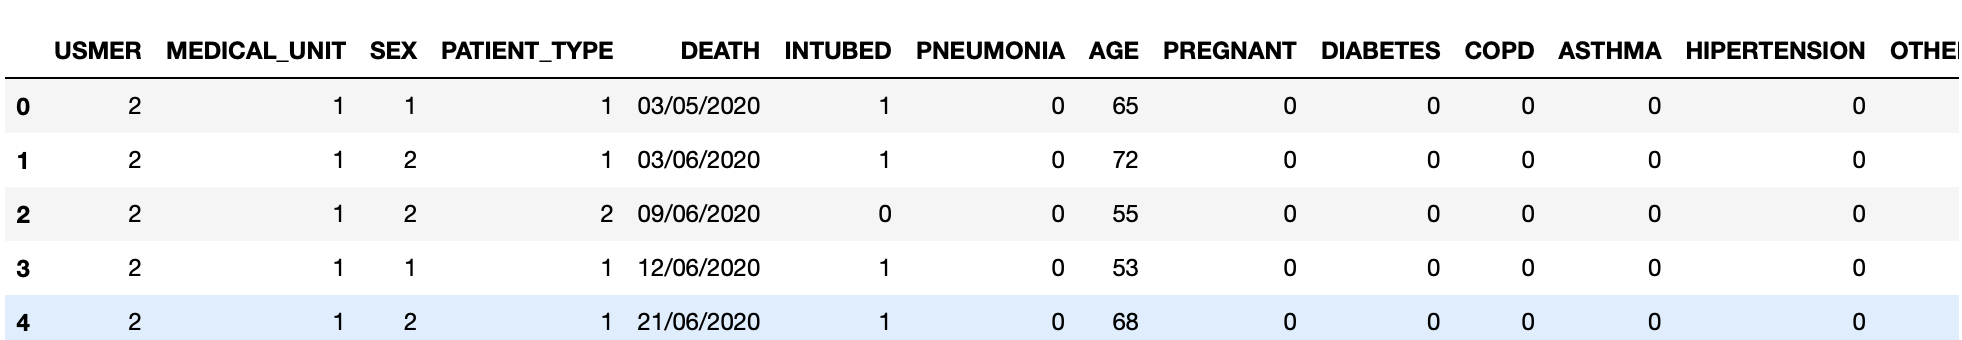
\includegraphics[width=1.0\textwidth]{image3.png}\newline
\end{center}
\end{itemize}

\subsection{Statystyki}
\indent{\large{
Średnia, minimalna i maksymalna wartość dla danej kolumny oraz odchylenie standardowe są podstawowymi danymi, które pozwolą nam wykryć ewentualne błędy.
}
\begin{lstlisting}
df_for_stats = df.iloc[:1000000]
cols_for_stats=cols
cols_for_stats.remove("DEATH")
for col in cols:
    print("For ",col,
          ":\nMean: ",df_for_stats[col].astype('int').mean(),
         "\nMin: ",df_for_stats[col].astype('int').min(),
         "\nMax: ",df_for_stats[col].astype('int').max(),
         "\nStd: ",df_for_stats[col].astype('int').std())
\end{lstlisting}
\begin{center}
    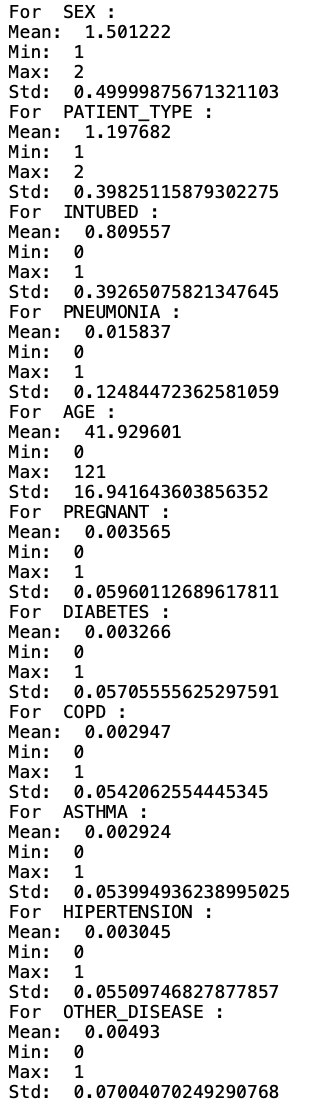
\includegraphics[width=0.4\textwidth]{image4.png}\newline
\end{center}
\subsection{Dane na wykresach}
\indent{\large{Aby baza danych była bardziej czytelna dla użytkownika została lekko zmodyfikowana.}}
\begin{lstlisting}
repSex = {1: "Female", 2: "Male"}
df.replace({"SEX": repSex},inplace=True)
df['AGE']=change(df['AGE'],[1,11,18,60],["Unknown","Child","Teenager","Adult","Senior"])
repDate={"9999-99-99":0}
df.replace({"DEATH":repDate},inplace=True)
df.loc[df["DEATH"] != 0,"DEATH"]=1
\end{lstlisting}
\newline
\large{Po tych zmianach tworzymy wykresy porównawcze.}
\begin{lstlisting}
new_cols=cols
new_cols.remove("SEX")
for x in new_cols:
    sns.set(style="whitegrid")
    ax = sns.countplot(y=x, hue="SEX", data=df)
    plt.ylabel(x)
    plt.title('Gender Plot')
    plt.show()
\end{lstlisting}
\begin{center}
    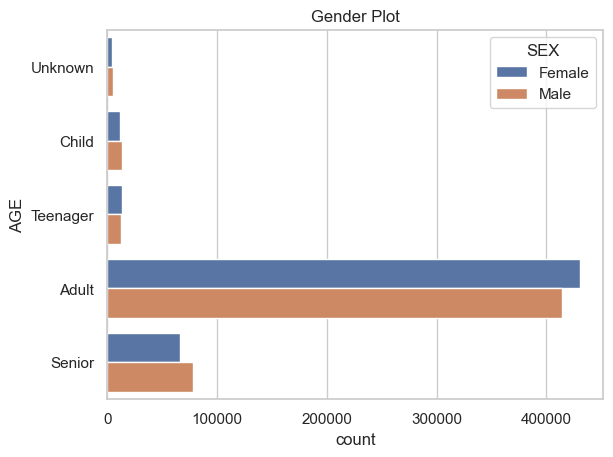
\includegraphics[width=0.9\textwidth]{image6.png}\newline
\end{center}
\begin{center}
    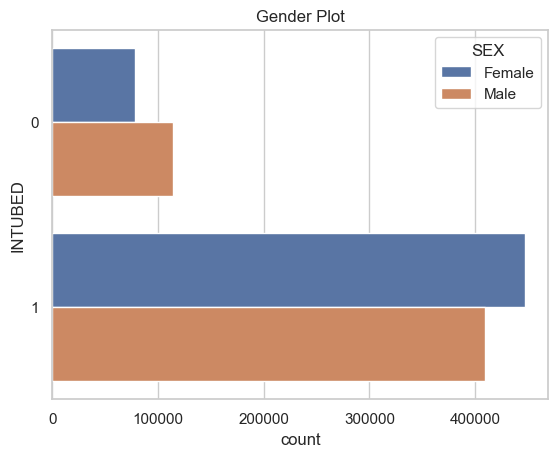
\includegraphics[width=0.8\textwidth]{image5.png}\newline
\end{center}
\begin{center}
    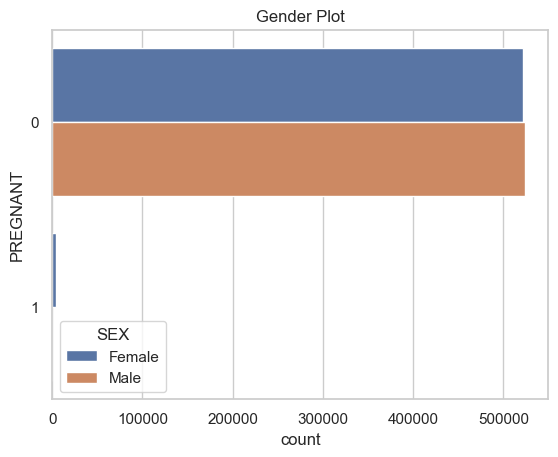
\includegraphics[width=0.8\textwidth]{image7.png}\newline
\end{center}
\section{\LARGE{Naive-Bayes}}
\subsection{Definicja}
\subsubsection{Czym jest?}
\large{Naiwny Bayes jest to klasyfikator probabilistyczny, który jest oparty na założeniu o wzajemnej niezależności predykatów. Polega na "uczeniu się" w trybie uczenia z nadzorem.\newline
\newline
Wyróżniamy trzy klasyfikatory w bibliotece scikit-learn:
\begin{itemize}
    \item Gaussian - dla danych ciągłych
    \item Multinomial - dla danych dyskretnych
    \item Bernoulli - dla danych binarnych
\end{itemize}
\newline
Model Bayesa używa metody maksymalnego prawdopodobieństwa. }
\subsubsection{Wzór}
\[ P(A|B) = \frac{P(B|A) \cdot P(A)}{ P(B)}\]\newline 
\begin{itemize}
    \item 
        P(A\textbar B) - prawdopodobieństwo, że A prawdziwe jeśli widzimy dowody na B
    \item P(B\textbarA) - prawdopodobieństwo, że B prawdziwe jeśli widzimy dowody na A
     \item P(B) - prawdopodobieństwo, że B prawdziwe 
      \item P(A) - prawdopodobieństwo, że B prawdziwe 
\end{itemize}
\newpage
\subsection{Kod}
\begin{lstlisting}
def naive_Bayes(X,y,typ):
    y.astype('int')
    X_train, X_test,y_train,y_test = train_test_split(X,y,test_size=0.2,random_state=7)
    model=typ
    clf=model.fit(X_train,y_train.astype('int'))
    pred_labels=model.predict(X_test)
    print("Classes: ",clf.classes_)
    print("\n*--------------------------------------------------*\n")
    if str(typ)=='GaussianNB()':
        print("Class Priors: ", clf.class_prior_)
    else:
        print("Class Priors: ", clf.class_log_prior_)
    score=model.score(X_test,y_test.astype('int'))
    print("\n*--------------------------------------------------*\n")
    print("Score: ",score)
    print("\n*--------------------------------------------------*\n")
    print('Training set score: {:.4f}'.format(model.score(X_train, y_train.astype('int'))))
    print('Test set score: {:.4f}'.format(model.score(X_test, y_test.astype('int'))))
    print("\n*--------------------------------------------------*\n")
    print( classification_report(y_test.astype('int'),pred_labels))
    print("\n*--------------------------------------------------*\n")
    y_pred = clf.predict(X_test)
    cm = confusion_matrix(y_test.astype('int'), y_pred.astype('int'))
    cm_matrix = pd.DataFrame(data=cm, columns=['Actual Positive:1', 'Actual Negative:0'], 
                                 index=['Predict Positive:1', 'Predict Negative:0'])
    sns.heatmap(cm_matrix, annot=True, fmt='d', cmap='YlGnBu')
    return X_train,X_test,y_train.astype('int'),y_test.astype('int'),clf,pred_labels
\end{lstlisting}
\newpage
\begin{itemize}
    \item Gaussian
    \begin{lstlisting}
X=df["OTHER_DISEASE"].values.reshape(-1,1)
y=df["DEATH"].values
X_train,X_test,y_train,y_test,clf,pred_labels,=naive_Bayes(X,y,GaussianNB())

    \end{lstlisting}
    \begin{center}
    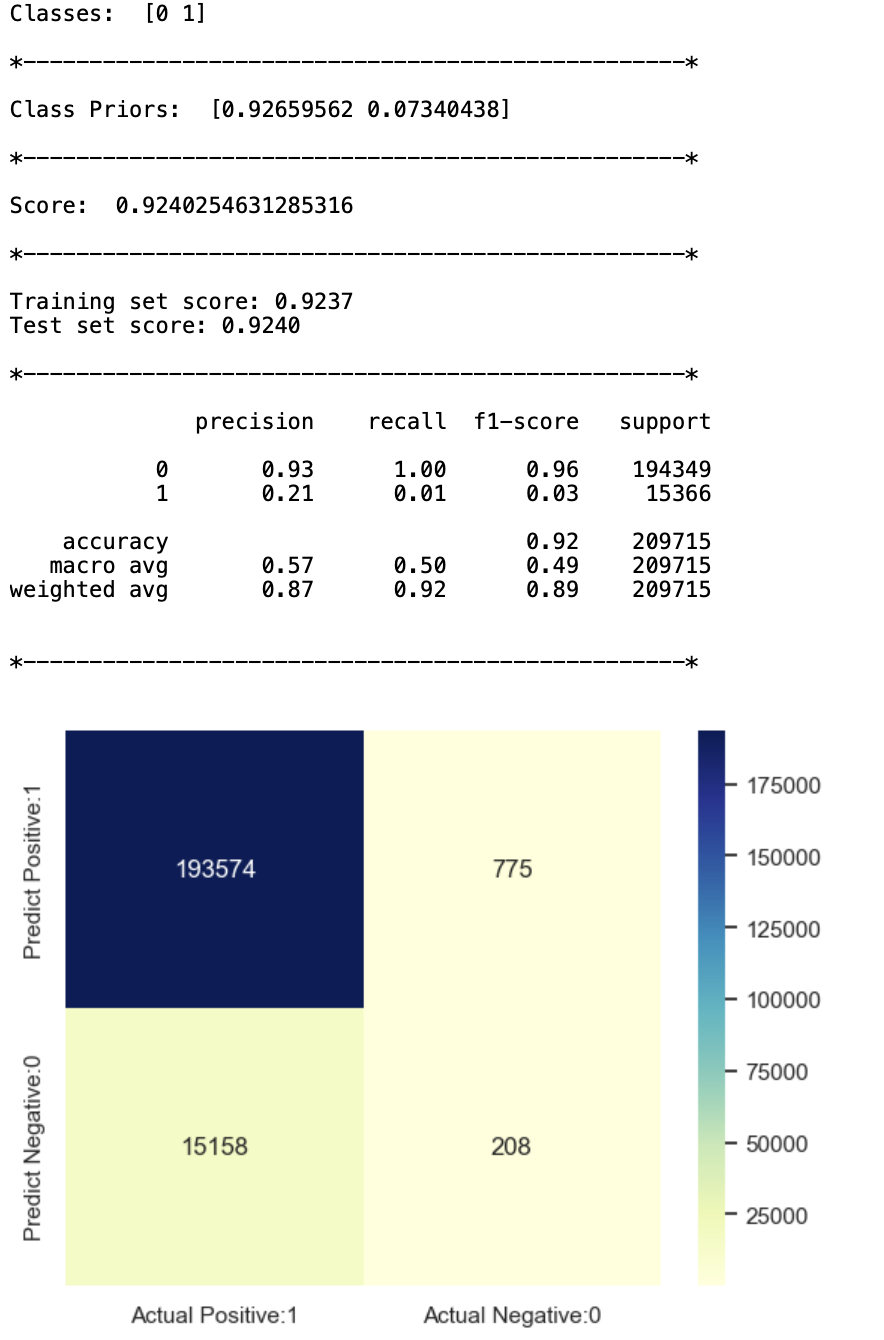
\includegraphics[width=0.7\textwidth]{image8.png}\newline
\end{center}
    \newpage
    \item Bernoulli
    \begin{lstlisting}
X=df["OTHER_DISEASE"].values.reshape(-1,1)
y=df["DEATH"].values
X_train,X_test,y_train,y_test,clf,pred_labels,=naive_Bayes(X,y,BernoulliNB())

    \end{lstlisting}
    \begin{center}
    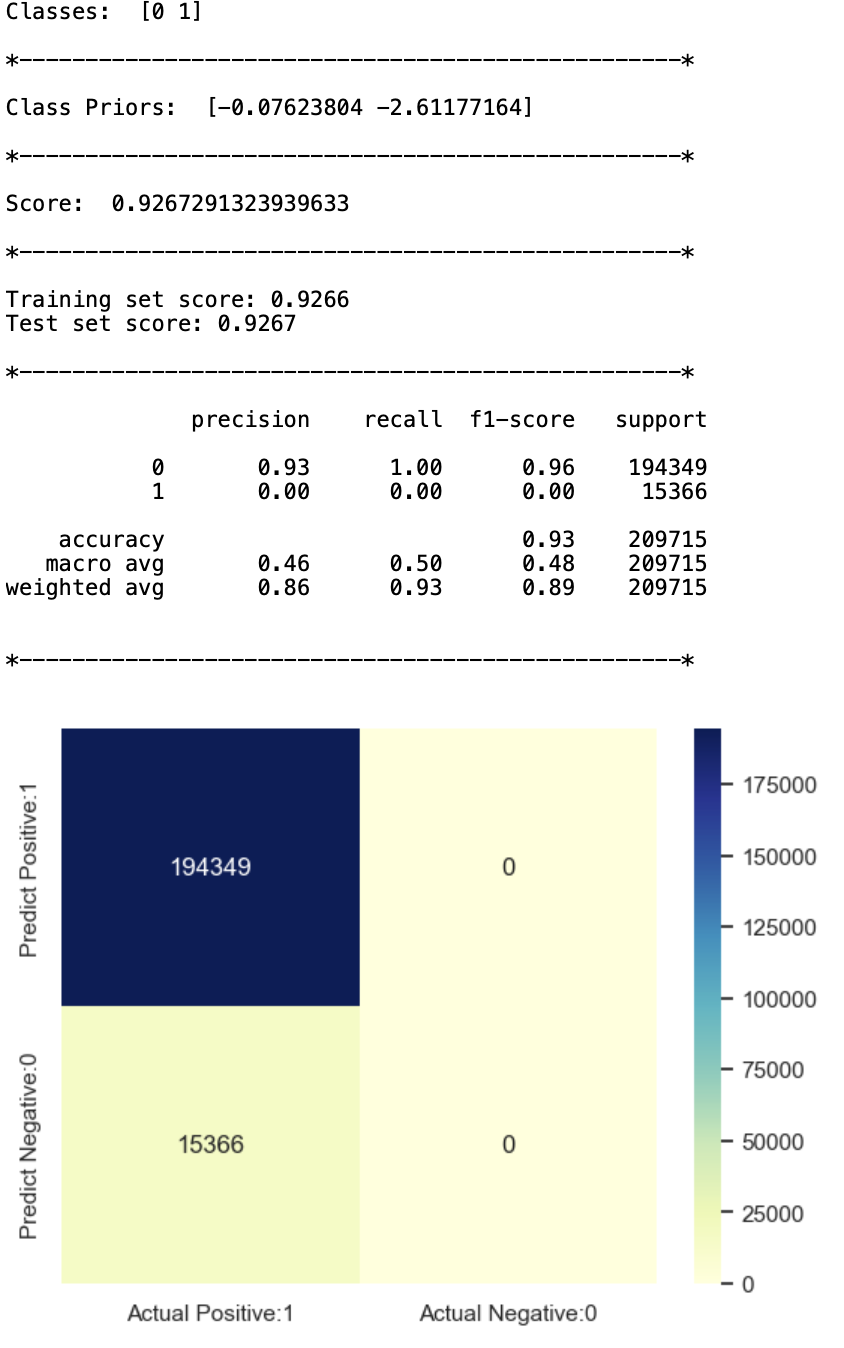
\includegraphics[width=0.7\textwidth]{image9.png}\newline
\end{center}
\end{itemize}
\newpage

\section{\LARGE{KNN}}
\subsection{Definicja}
\large{Metoda K najbliższych sąsiadów należy do grupy algorytmów leniwych. Polega na podporządkowaniu danej obserwacji taką klasę, która ma najwięcej podobnych próbek. \newline\newline
Ciekawym przykładem może być klasyfikacja czy dany człowiek skłamał poprzez ewaulacje pulsu wraz z badaniami galwanometrem.}
    \begin{center}
    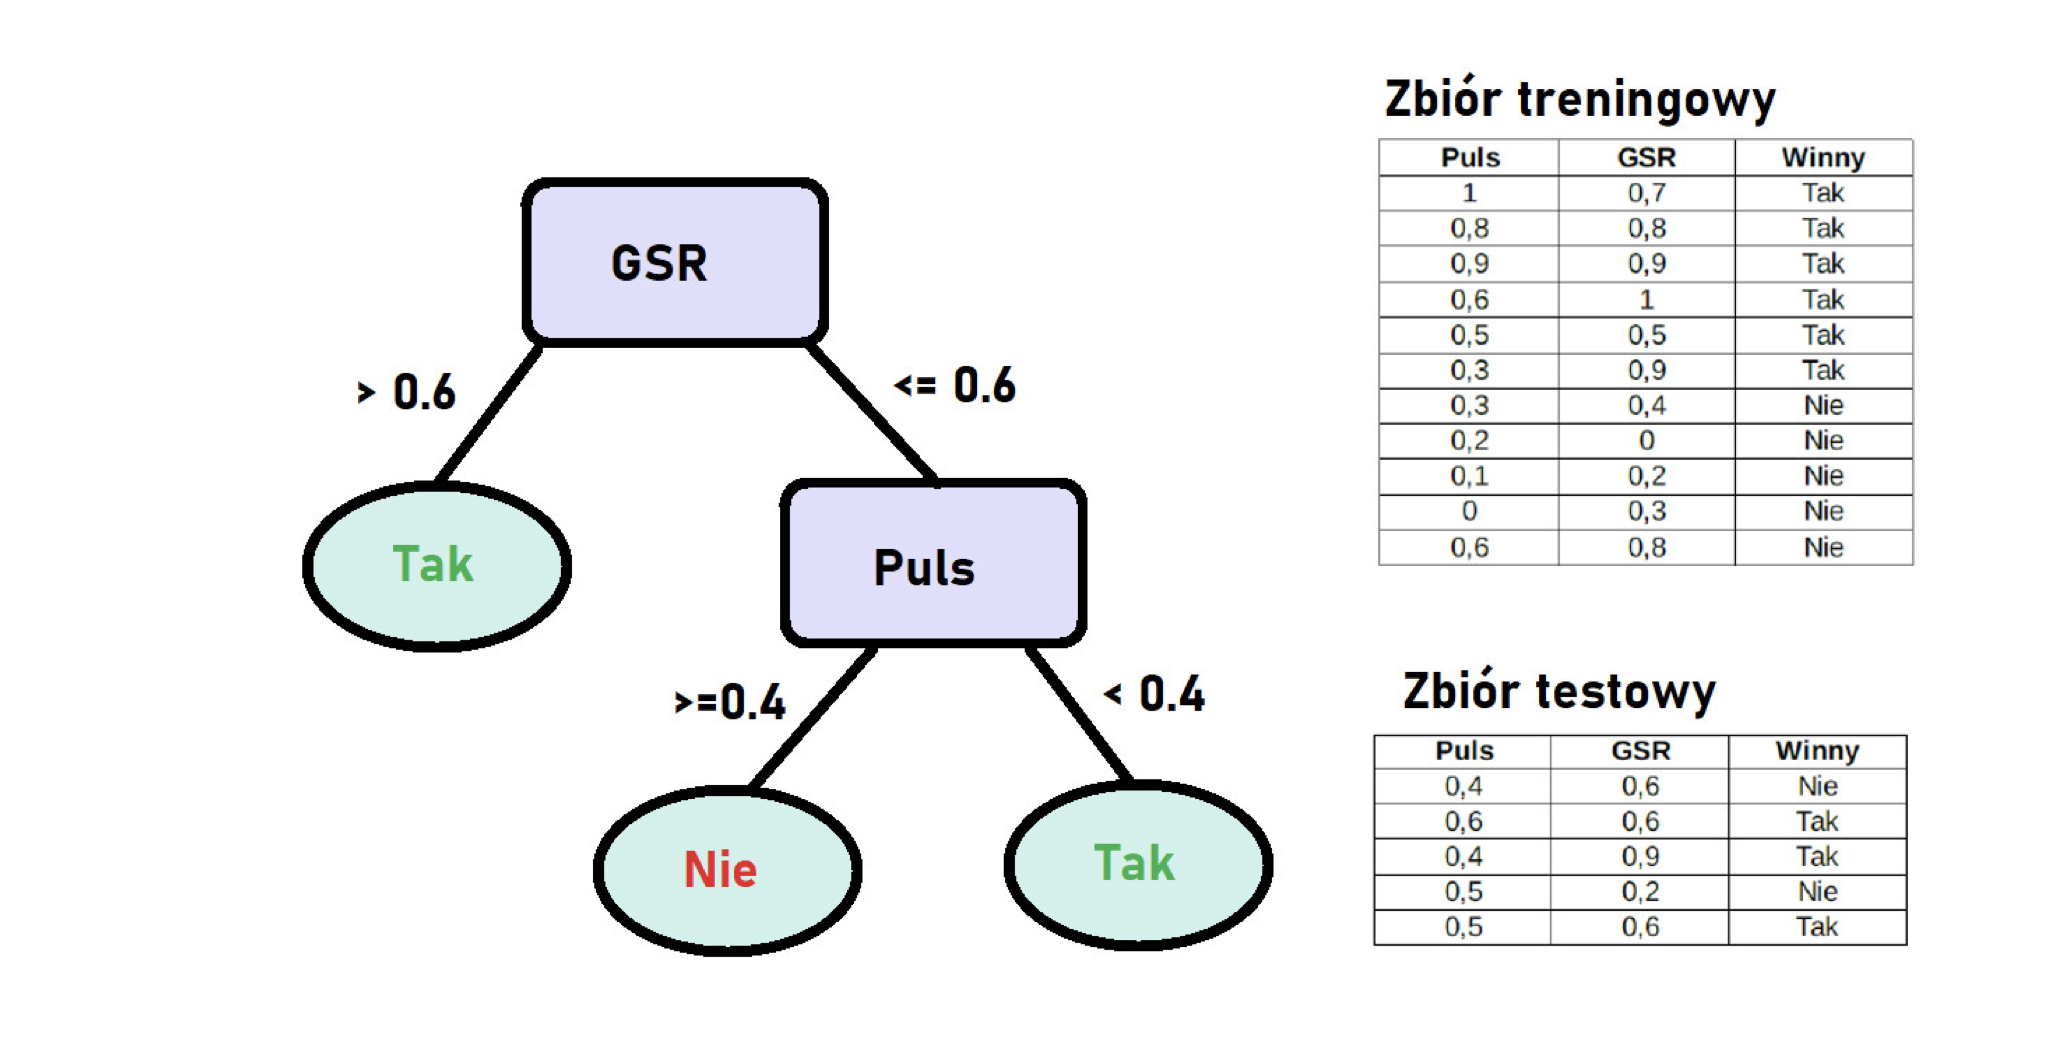
\includegraphics[width=1.0\textwidth]{puls.png}\newline
\end{center}
\newpage
\subsection{Kod}
\begin{lstlisting}
def knn(X,Y):
    X_train, X_test, Y_train, Y_test = train_test_split(X,Y,test_size=0.3,random_state=10)
    knn_model = KNeighborsClassifier()
    knn_model.fit(X_train, Y_train.astype("int"))
    Y_predict_knn = knn_model.predict(X_test)
    #Comparing the output I expected (Y_test) against the ones the model predicted (Y_predict)
    knn_metrics = metrics.classification_report(Y_test.astype("int"),Y_predict_knn.astype("int"))
    print(knn_metrics)
    table = pd.DataFrame(Y_test.astype("int"))
    print('table 1')
    print(table.head())
    #add the predictions to the dataframe
    table['predictions'] = Y_predict_knn.astype("int")
    print('table 2')
    print(table.head())
    accuracy_knn = accuracy_score(Y_test.astype("int"),Y_predict_knn.astype("int"))
    precision_knn = precision_score(Y_test.astype("int"), Y_predict_knn.astype("int"))
    f1_knn = f1_score(Y_test.astype("int"),Y_predict_knn.astype("int"))
    recall_knn = recall_score(Y_test.astype("int"), Y_predict_knn.astype("int"))
    print(precision_knn)
    print(accuracy_knn)
    print(f1_knn)
    print(recall_knn)
    plt.bar(['Accuracy','F1 Score','Recall Score','Precision Score'],[accuracy_knn,f1_knn,recall_knn,precision_knn],color=['red','green','purple','orange'])
    plt.plot([accuracy_knn,f1_knn,recall_knn,precision_knn],color='black')
    plt.title('Evaluation Metrics for K-Nearest Neighbors')
    plt.show()
    cm = confusion_matrix(Y_test.astype('int'), Y_predict_knn.astype('int'))
    cm_matrix = pd.DataFrame(data=cm, columns=['Actual Positive:1', 'Actual Negative:0'], 
                                 index=['Predict Positive:1', 'Predict Negative:0'])
    sns.heatmap(cm_matrix, annot=True, fmt='d', cmap='YlGnBu')

\end{lstlisting}

    \begin{lstlisting}
knn(X=df["OTHER_DISEASE"].iloc[:100000].values.reshape(-1,1),
Y = df["DEATH"].iloc[:100000].values)

    \end{lstlisting}
    \begin{center}
    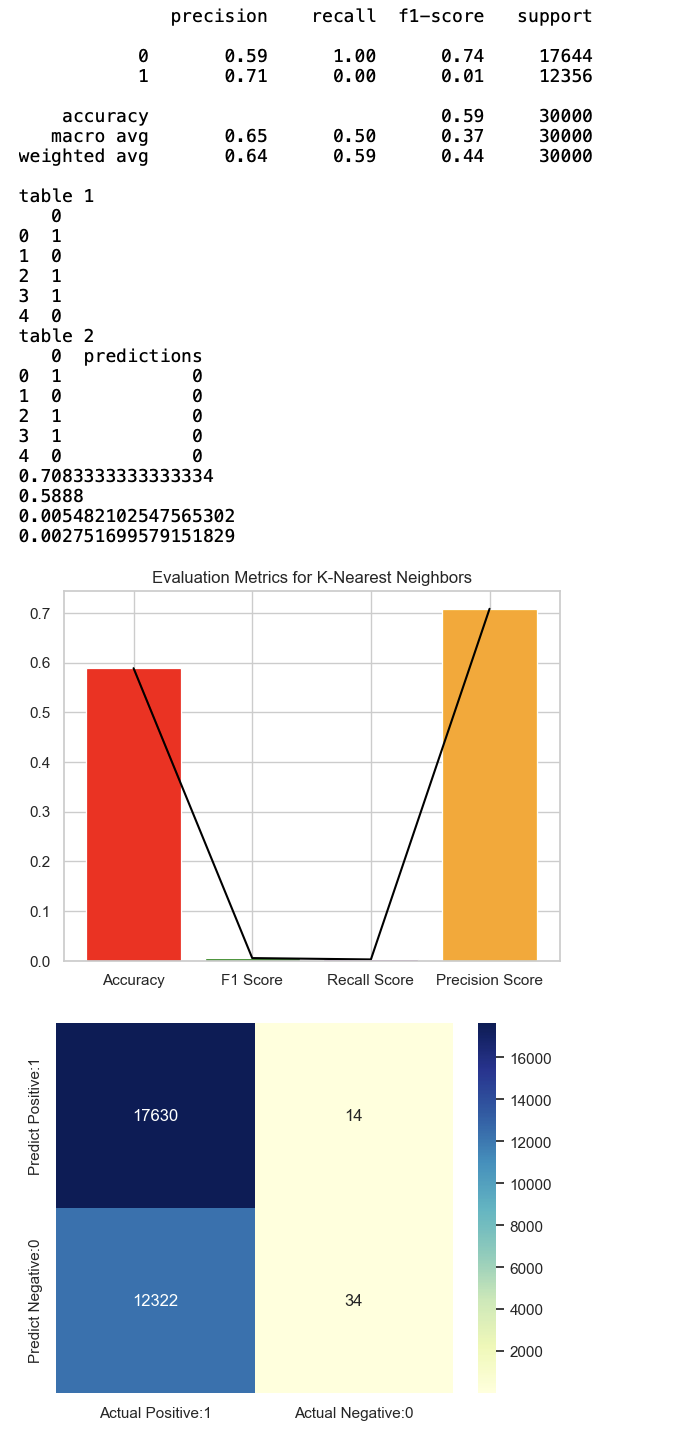
\includegraphics[width=0.6\textwidth]{image10.png}\newline
\end{center}
\newpage

\section{\LARGE{Decision-Tree}}
\subsection{Definicja}
Drzewo decyzyjne jest to jeden ze sposobów klasyfikacji, polegający na podejmowaniu decyzji na podstawie pytań. Przykładem może byc klasyfikacja czy człowiek zdrowo się odżywia.
    \begin{center}
    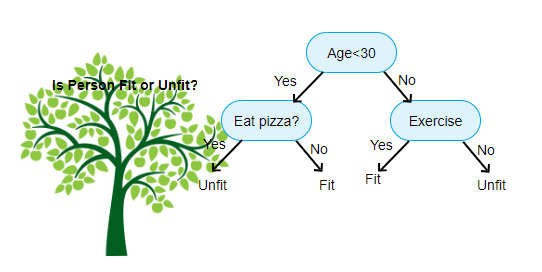
\includegraphics[width=0.7\textwidth]{is.png}\newline
\end{center}
\subsection{Kod}
\begin{lstlisting}
X=df["OTHER_DISEASE"].iloc[:100000].values.reshape(-1,1)
y = df["DEATH"].iloc[:100000].values.astype("int")
X_train, X_test, y_train, y_test = train_test_split(X, y, test_size=0.3, random_state=1)
clf = tree.DecisionTreeClassifier()
clf = clf.fit(X_train,y_train)
y_pred = clf.predict(X_test)
tree.plot_tree(clf)
dot_data = StringIO()
export_graphviz(clf, out_file=dot_data,  
                filled=True, rounded=True,
                special_characters=True,feature_names = ["OTHER_DISEASE"],class_names=['0','1'])
graph = pydotplus.graph_from_dot_data(dot_data.getvalue())  
graph.write_png('covid_DT1.png')
Image(graph.create_png())
\end{lstlisting}

    \begin{center}
    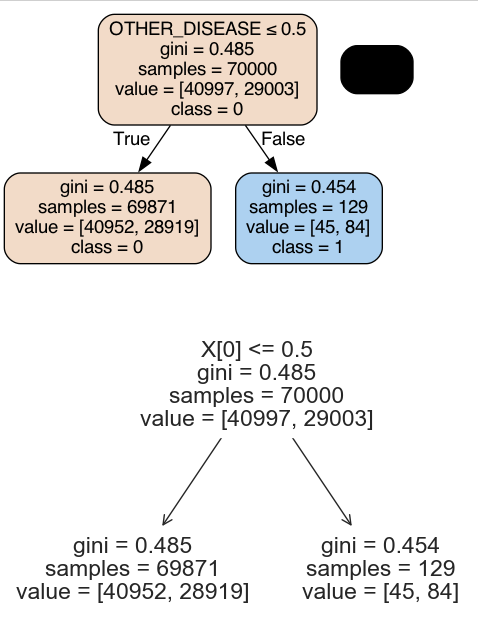
\includegraphics[width=0.5\textwidth]{image11.png}\newline
\end{center}

\section{\LARGE{Neural-Networks}}
\subsection{Definicja}
\large{Sieci neuronowe wzorowane są na budowie biologicznego systemu neuronowego w ujęciu matematyczno- informatycznym są grafem skierowanym.}
    \begin{center}
    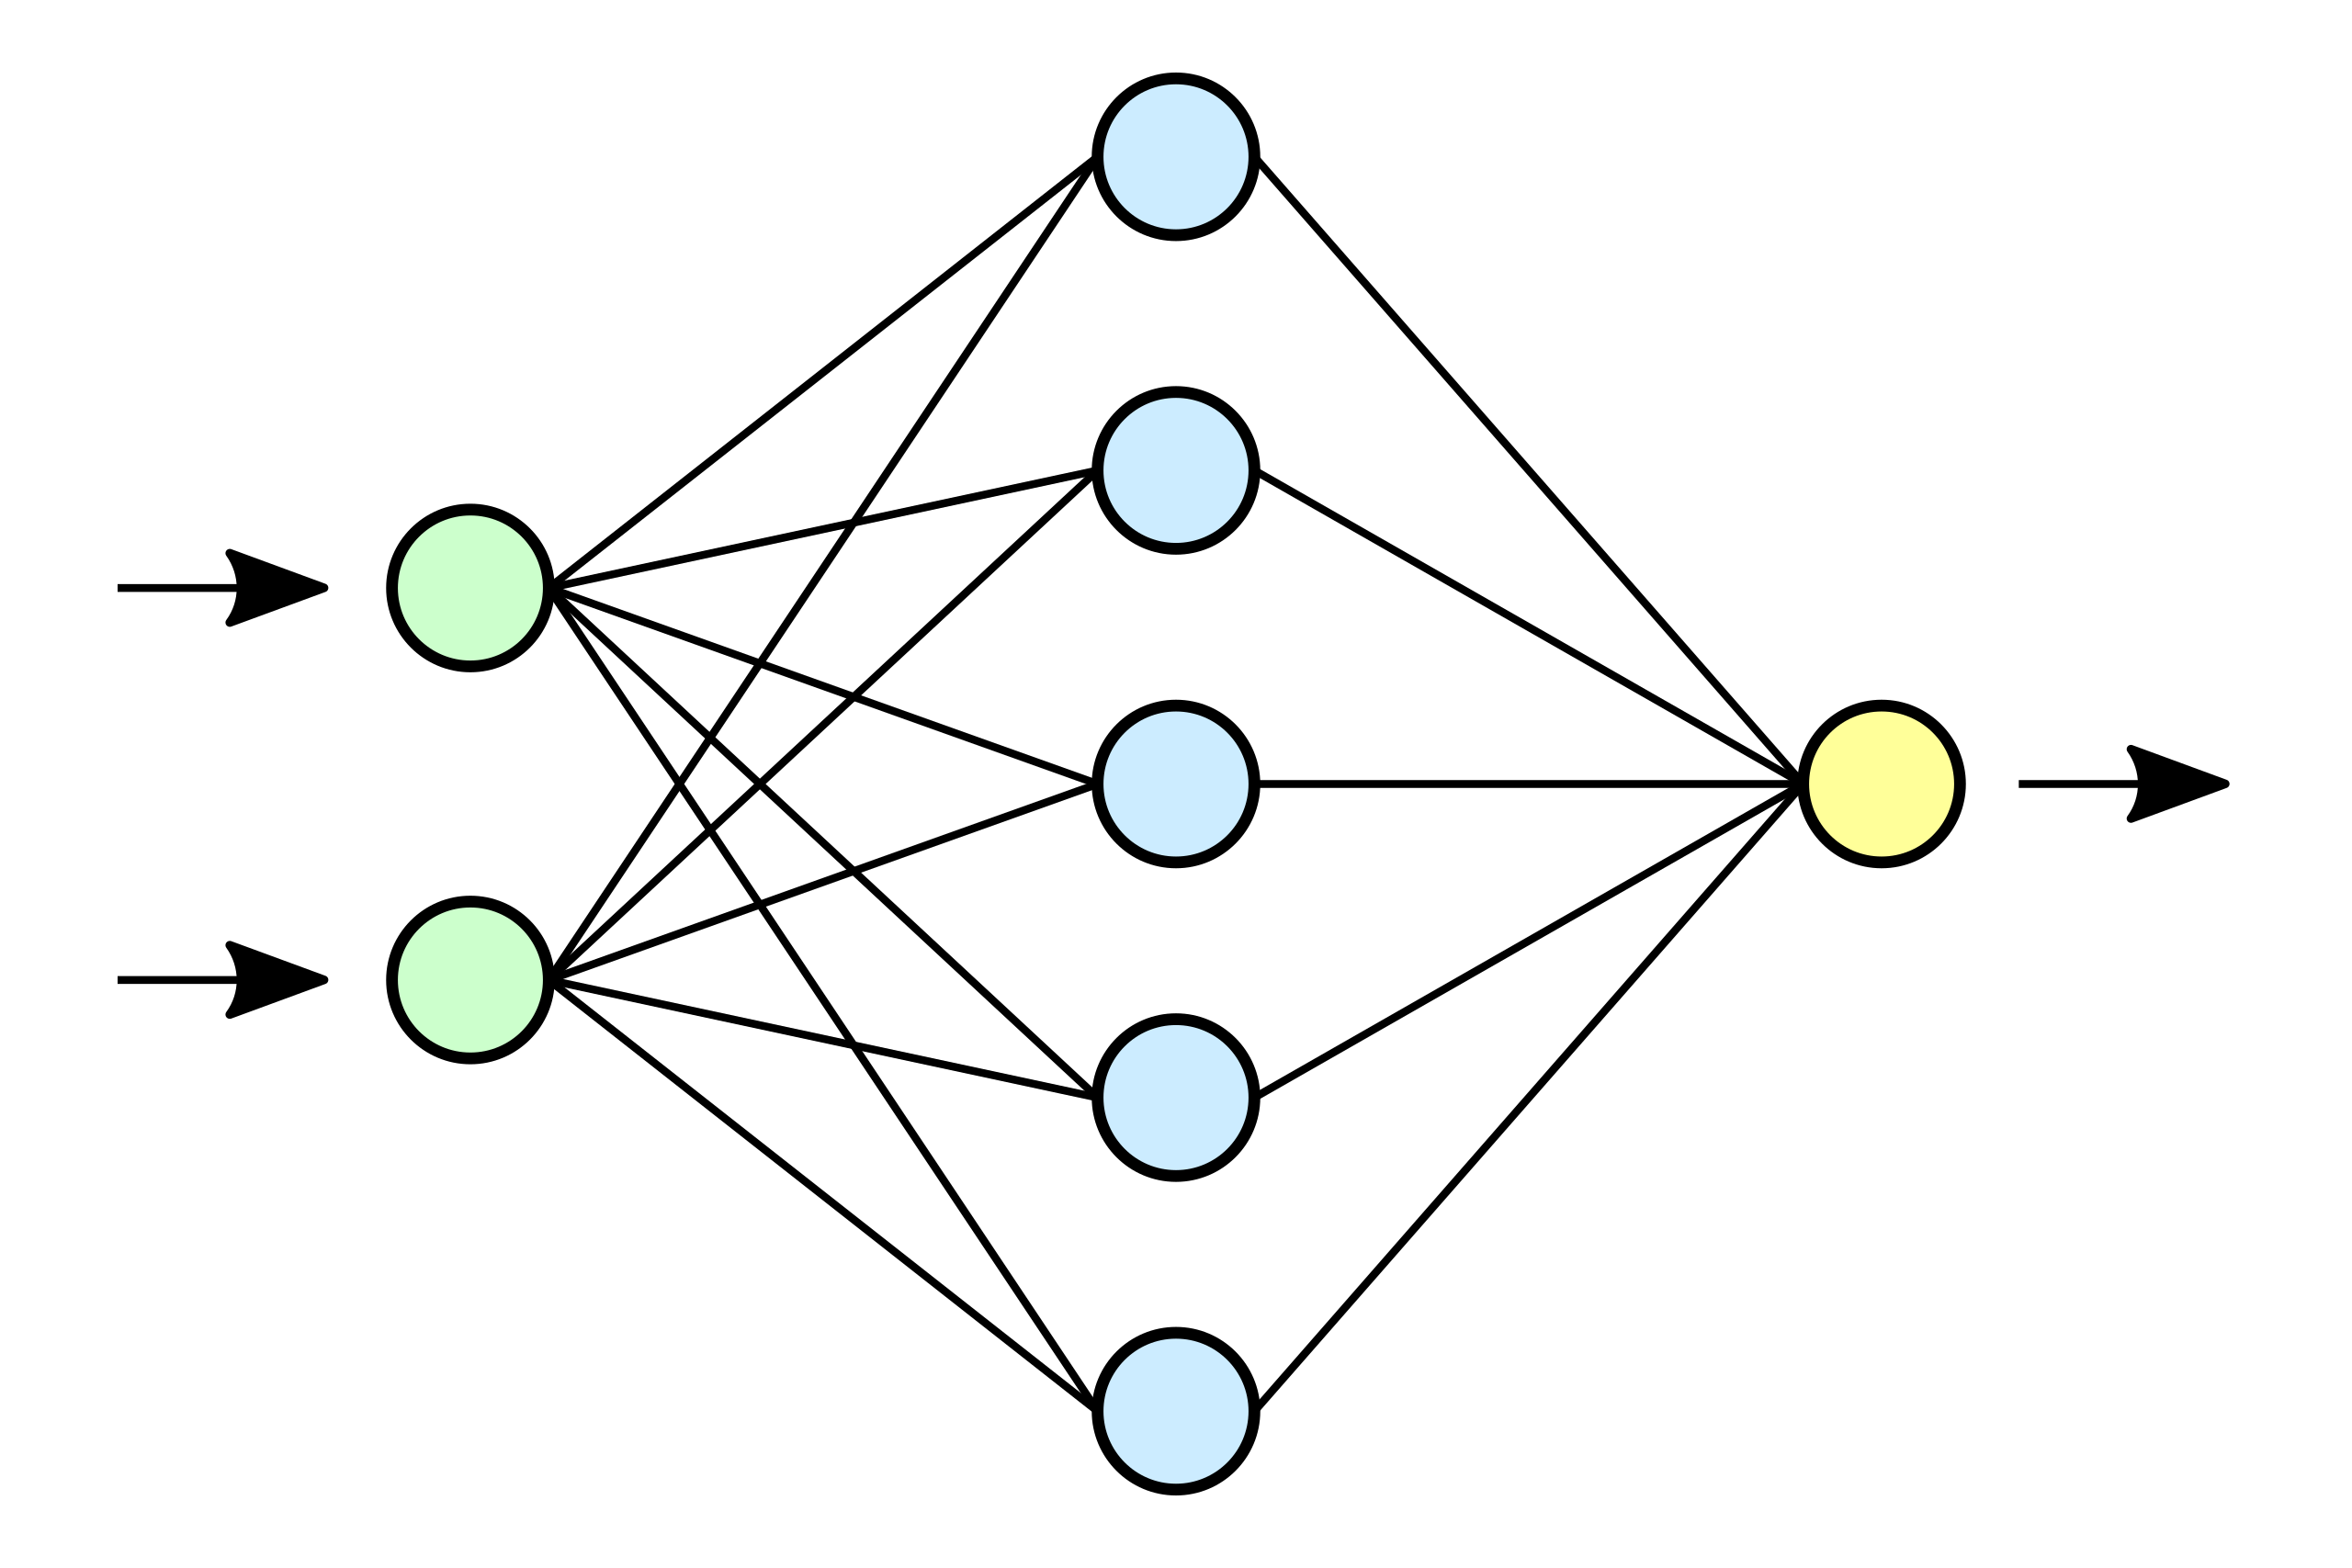
\includegraphics[width=0.5\textwidth]{neuron.png}\newline
\end{center}
\newpage
\subsection{Kod}
\begin{lstlisting}
def neural_network():
    scaler = StandardScaler()

    scaler.fit(X_train)

    train_data = scaler.transform(X_train)
    test_data = scaler.transform(X_test)
    print(train_data[:3])

    mlp = MLPClassifier(hidden_layer_sizes=(10, 10), max_iter=1000)

    mlp.fit(train_data, y_train)

    predictions_train = mlp.predict(train_data)
    predictions_test = mlp.predict(test_data)
    percent = (mlp.score(test_data, y_test))

    return ["Neural Network", percent, mlp]

r=neural_network()
plot_confusion_matrix(r[2],X_test,y_test)
\end{lstlisting}

    \begin{center}
    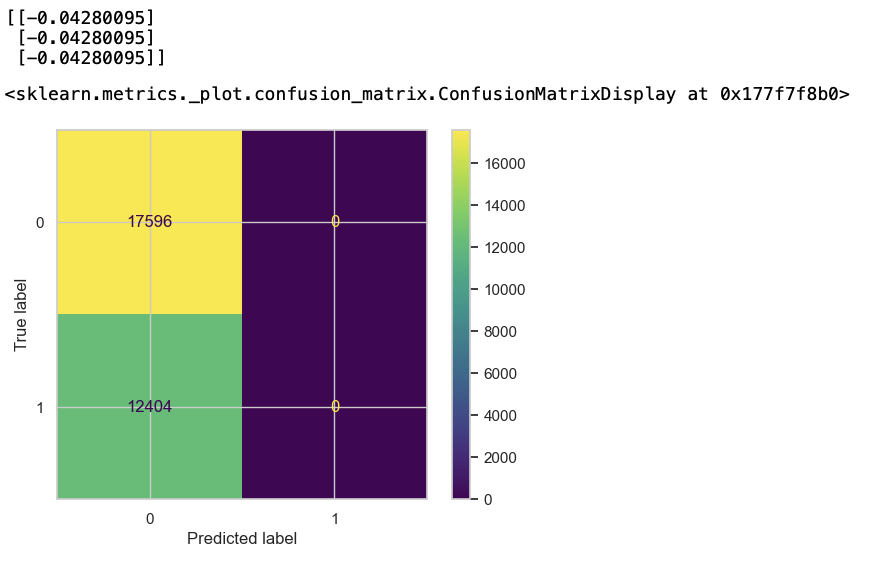
\includegraphics[width=1.0\textwidth]{image12.png}\newline
\end{center}
\newpage
\section{\LARGE{Apriori}}
\subsection{Definicja}
Reguły asocjacyjne polegają na ocenie wiarygodności jakiejś reguły. Najlepiej wytłumaczyć takie reguły na bazie danych:
\newline
    \begin{center}
    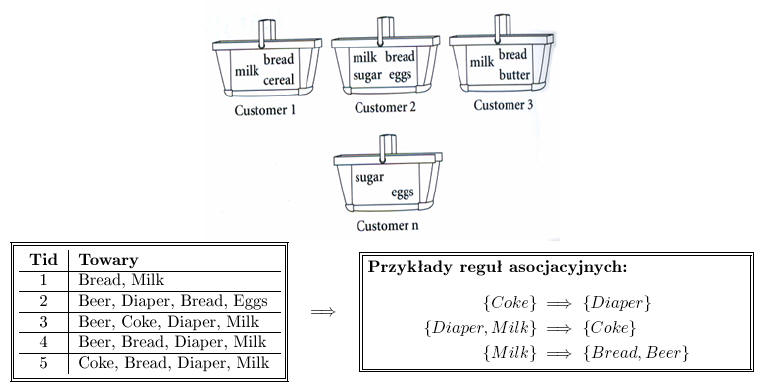
\includegraphics[width=1.0\textwidth]{regu.png}\newline
\end{center}
\newline
\large{„Kiedy kupimy pieluche i mleko, wtedy też kupimy piwo" - stwierdzenie to jest prawdziwe tylko dla 3 i 4, a 5 nie zawiera piwa więc wiarygoność jest równa 2/3.}
    \begin{center}
    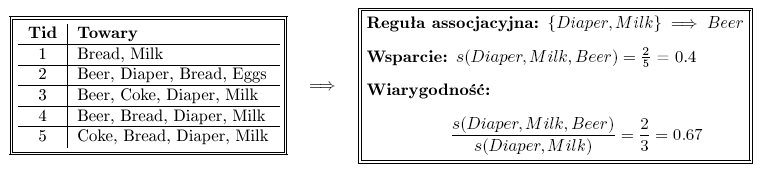
\includegraphics[width=1.0\textwidth]{re2.png}\newline
\end{center}
\newpage
\subsection{Kod}
\newline\newline
\large{Aby rozpocząć trzeba przygotować baze danych. Wartości stają się kolumnami:}
\newline\newline
\begin{lstlisting}
data = []
df_te=df.iloc[:1000]
for i in range(0, df_te.shape[0]-1):
    data.append([str(df_te.values[i,j]) for j in range(0, df_te.shape[1])])

    
th = TransactionEncoder()
th_arr = th.fit(data).transform(data)
new_df = pd.DataFrame(th_arr,columns=th.columns_)
new_df.head()
\end{lstlisting}

    \begin{center}
    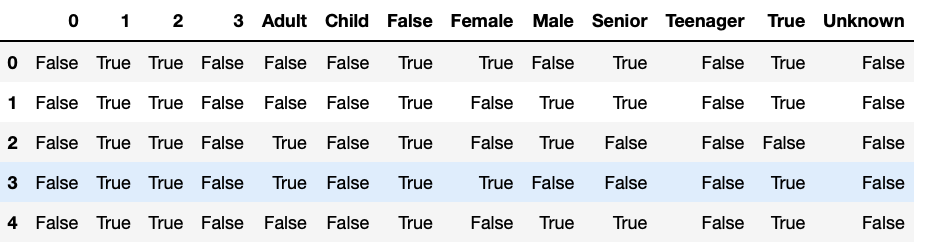
\includegraphics[width=0.7\textwidth]{image13.png}\newline
\end{center}
\newline\newline
\large{Wyniki aprori:}
\newline\newline
\begin{lstlisting}
apr = apriori(new_df,min_support = 0.2, use_colnames = th.columns_)
apr.head()
\end{lstlisting}

    \begin{center}
    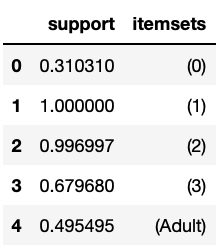
\includegraphics[width=0.4\textwidth]{image14.png}\newline
\end{center}

\large{Uruchamianie eksploracji reguł z konfiguracją:}
\begin{lstlisting}
config = [ ('antecedent support',0.7),('confidence',0.8),('conviction',3)]
for metric, new_th in config:
    rules = association_rules(apr, metric = metric, min_threshold=new_th)
    if rules.empty:
        print("Dataframe is Empty")
    print(rules.columns.values)
    print("My configuration: ", metric, " : ",new_th)
    print(rules)
    
    support = rules.loc[:,"support"]
    confidence = rules.loc[:,'confidence']
    plt.scatter(support,confidence,edgecolors="blue")
    plt.xlabel('support')
    plt.ylabel('confidence')
    plt.title(metric+' : ' +str(new_th))
    plt.savefig('plot%03s.png'%(metric))
\end{lstlisting}
    \begin{center}
    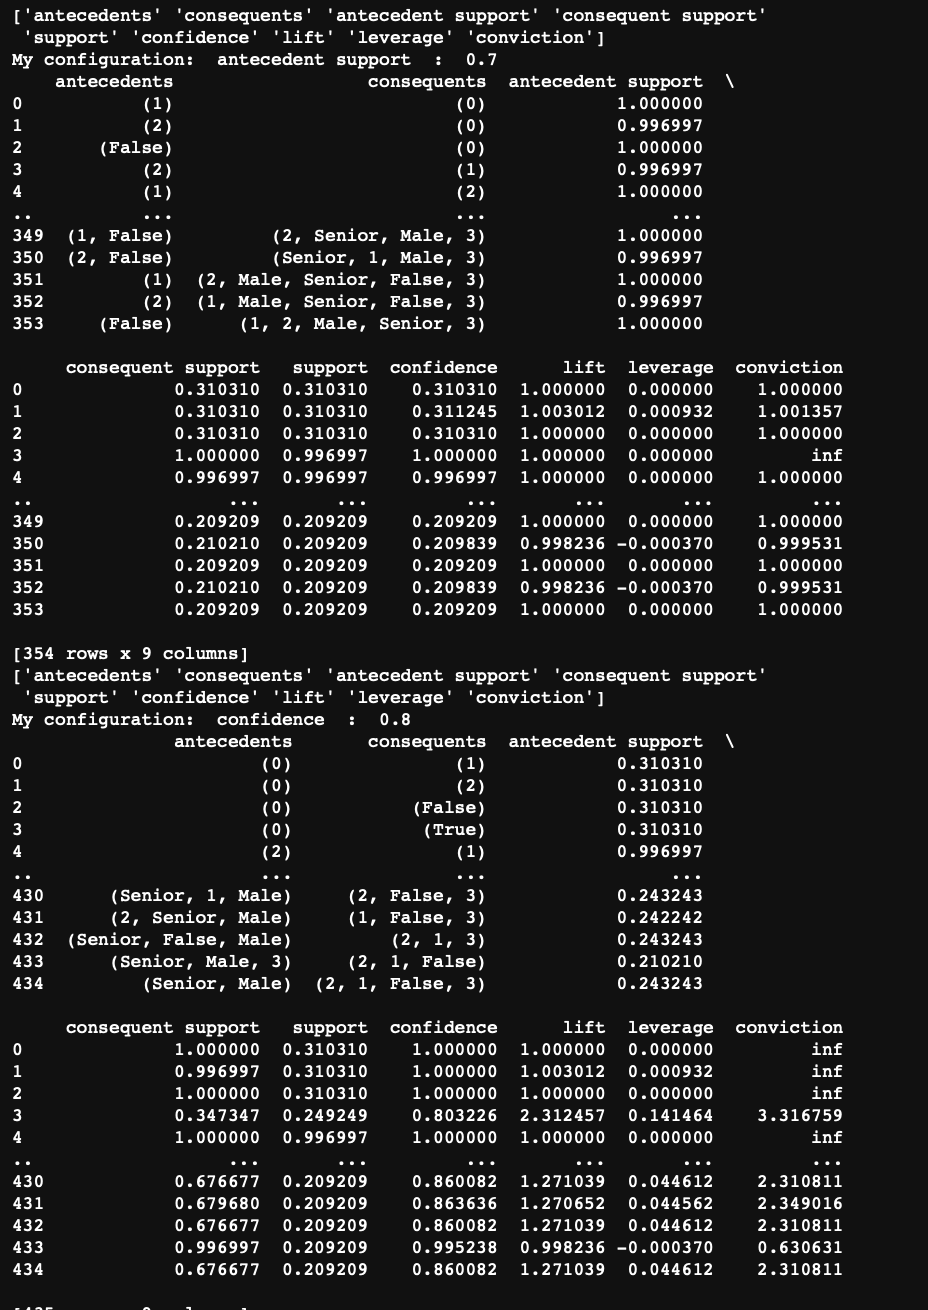
\includegraphics[width=0.8\textwidth]{image15.png}\newline
\end{center}
    \begin{center}
    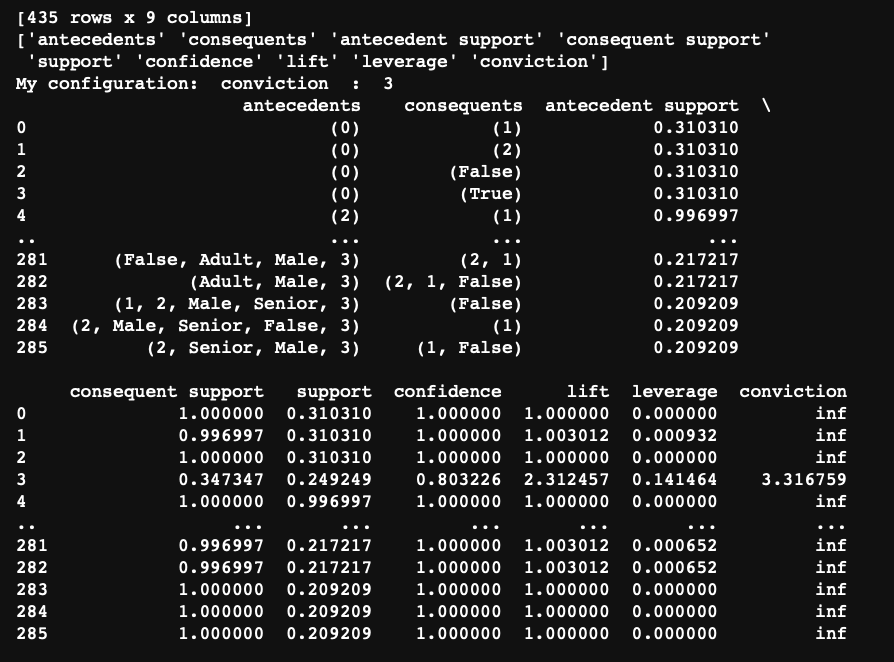
\includegraphics[width=0.8\textwidth]{image16.png}\newline
\end{center}
    \begin{center}
    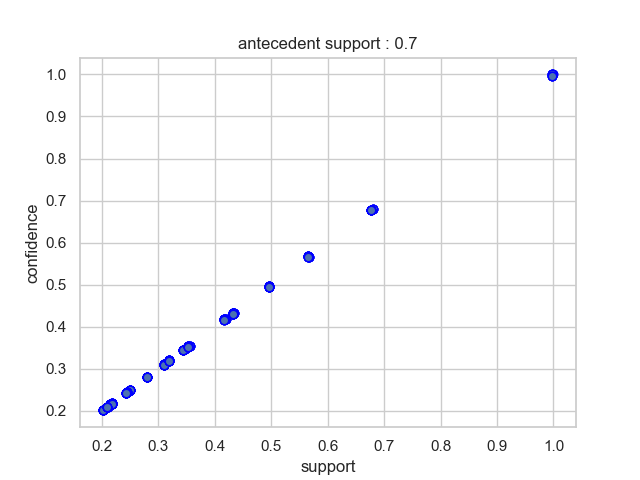
\includegraphics[width=0.8\textwidth]{1.png}\newline
\end{center}
    \begin{center}
    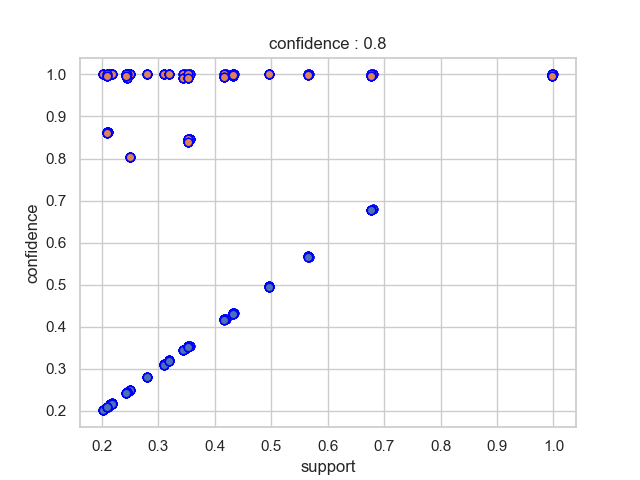
\includegraphics[width=0.8\textwidth]{2co.png}\newline
\end{center}
    \begin{center}
    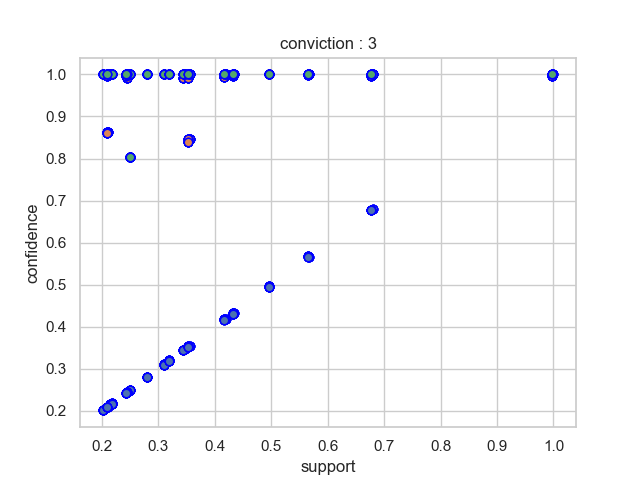
\includegraphics[width=0.8\textwidth]{3convi.png}\newline
\end{center}
\newpage
\large{Reguły:}
\begin{lstlisting}
print(rules[rules['antecedents']==frozenset({'Female'})].to_string())
print("\n-------------------------------------------\n")
print(rules[rules['antecedents']==frozenset({'Male'})].to_string())
print("\n-------------------------------------------\n")
print(rules[rules['antecedents']==frozenset({'Senior'})].to_string())
print("\n-------------------------------------------\n")
\end{lstlisting}
    \begin{center}
    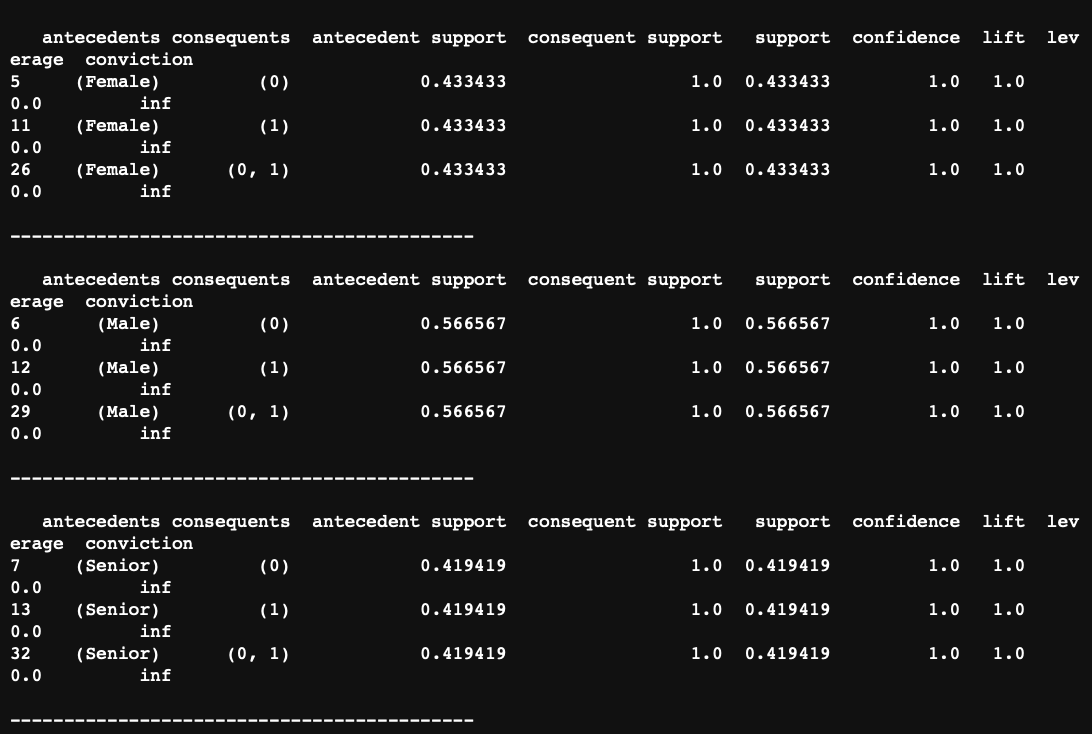
\includegraphics[width=0.7\textwidth]{image17.png}\newline
\end{center}
\newpage
\section{\LARGE{Link do githuba}}
Cały projekt będący elementem mojej pracy został wstawiony na githuba  \url{https://github.com/komolcia/INF-D-2023-Julia-Komorowska-266386} oraz opisany  w README.md.
\section{\LARGE{Bibliografia}}
\begin{itemize}
    \item \url{https://www.kaggle.com/code/bhanuchanderu/data-mining-a-demo-with-titanic-data/notebook} - Apriori
    \item \url{https://towardsdatascience.com/naive-bayes-classifier-how-to-successfully-use-it-in-python-ecf76a995069} - Naive Bayes
    \item \url{https://pl.wikipedia.org/wiki/Naiwny_klasyfikator_bayesowski} - definicja Naiwnego Bayesa
    \item \url{https://www.kaggle.com/code/prashant111/knn-classifier-tutorial} -KNN
    \item \url{https://scikit-learn.org/stable/modules/neural_networks_supervised.html}- Neural Networks
\end{itemize}
\end{document}
